\documentclass[11pt, a4paper]{article}
\usepackage[none]{hyphenat}
\sloppy
\usepackage[left=1cm, right=1cm, top=1cm, bottom=2cm]{geometry}
\parindent 0px % indent new lines by 0 pixels
\usepackage[utf8]{inputenc}
\usepackage{hyperref, amsfonts,amssymb,amsmath,tikz,pgfplots,float,graphicx,tabularx,array,siunitx,cleveref}
\usetikzlibrary{angles,quotes,positioning}
\usetikzlibrary{decorations.markings}

%\hypersetup{
%	colorlinks=true,    % Use colored text instead of boxes
%	linkcolor=blue,     % Color for internal links (TOC, \cref)
%	citecolor=blue,    % Color for citations (optional)
%	urlcolor=blue   % Color for URLs (optional)
%}

\def\ParagraphSpacing{30pt}
\allowdisplaybreaks % lets aligned equations flow through multiple pages.

\title{\small AS91522 - Physics 3.2\\ \huge Circular Motion of a Stunt Glider}
\author{Nathan Tasker}
\date{\today}

\begin{document}
	\maketitle
	\tableofcontents
	\newpage
	\section{Vertical Circle: Loop the loop including Dip and Arch}
	\subsection{Achieved}
	During motion, 3 forces are acting on the stunt glider:
	\begin{enumerate}
		\item Gravity ($\vec{F_g}$) (i.e. Weight) always vertically downwards (i.e. toward center of Earth).
		\item Lift ($\vec{F_L}$) perpendicular to direction of velocity, toward the center of the circular path.
		\item Air Resistance ($\vec{F_R}$) (i.e. Friction, Drag) opposite to direction of velocity.
	\end{enumerate}
	\vspace{\ParagraphSpacing}
	The force of gravity is always constant in both magnitude and direction (vertically downwards) regardless of the glider's velocity or position in the loop (top, bottom, and anywhere else). This is because $|\vec{F_g}|=mg$ where mass ($m$) and the acceleration of gravity ($g$) are constants.\\[\ParagraphSpacing]
	Conversely, the force of lift varies in both direction and magnitude as the glider performs the loop the loop.\\
	Lift's magnitude ($|\vec{F_L}|$) is greatest at the bottom, $\because |\vec{F_L}|=\frac{1}{2}p|\vec{v}|^2AC_L$, $\therefore |\vec{F_L}|\propto v^2$. Because velocity is greatest at bottom, lift force is as well. To maintain circular motion the centripetal force ($|\vec{F_c}|=|\vec{F_L}|-|\vec{F_g}|$) towards the center of the circular path must have a magnitude value great enough to provide necessary centripetal acceleration for the circular path radius, meaning the lift force upwards must at least be greater than the gravity force downwards ($|\vec{F_L}|>|\vec{F_g}|$ in order for $|\vec{F_c}|>0$).\\
	Lift's magnitude ($|\vec{F_L}|$) is least at the top, because the direction of gravity force is toward the center of the circular path. This means ($|\vec{F_c}|=|\vec{F_L}|+|\vec{F_g}|$).\\
	\begin{figure}[H]
		\centering
		\begin{tikzpicture}
			\pgfmathsetmacro{\TextGap}{0.2};
			\pgfmathsetmacro{\HalfWidth}{8};
			\pgfmathsetmacro{\TopLineY}{3.05};
			\pgfmathsetmacro{\BottomLineY}{-2.65};
			\coordinate(BottomPos1) at (-5.65,\TopLineY);
			\coordinate(TopPos) at (-0.1,-2.58);
			\coordinate(BottomPos2) at (5.6,2.9);
			\node[inner sep=0] at (0,0) {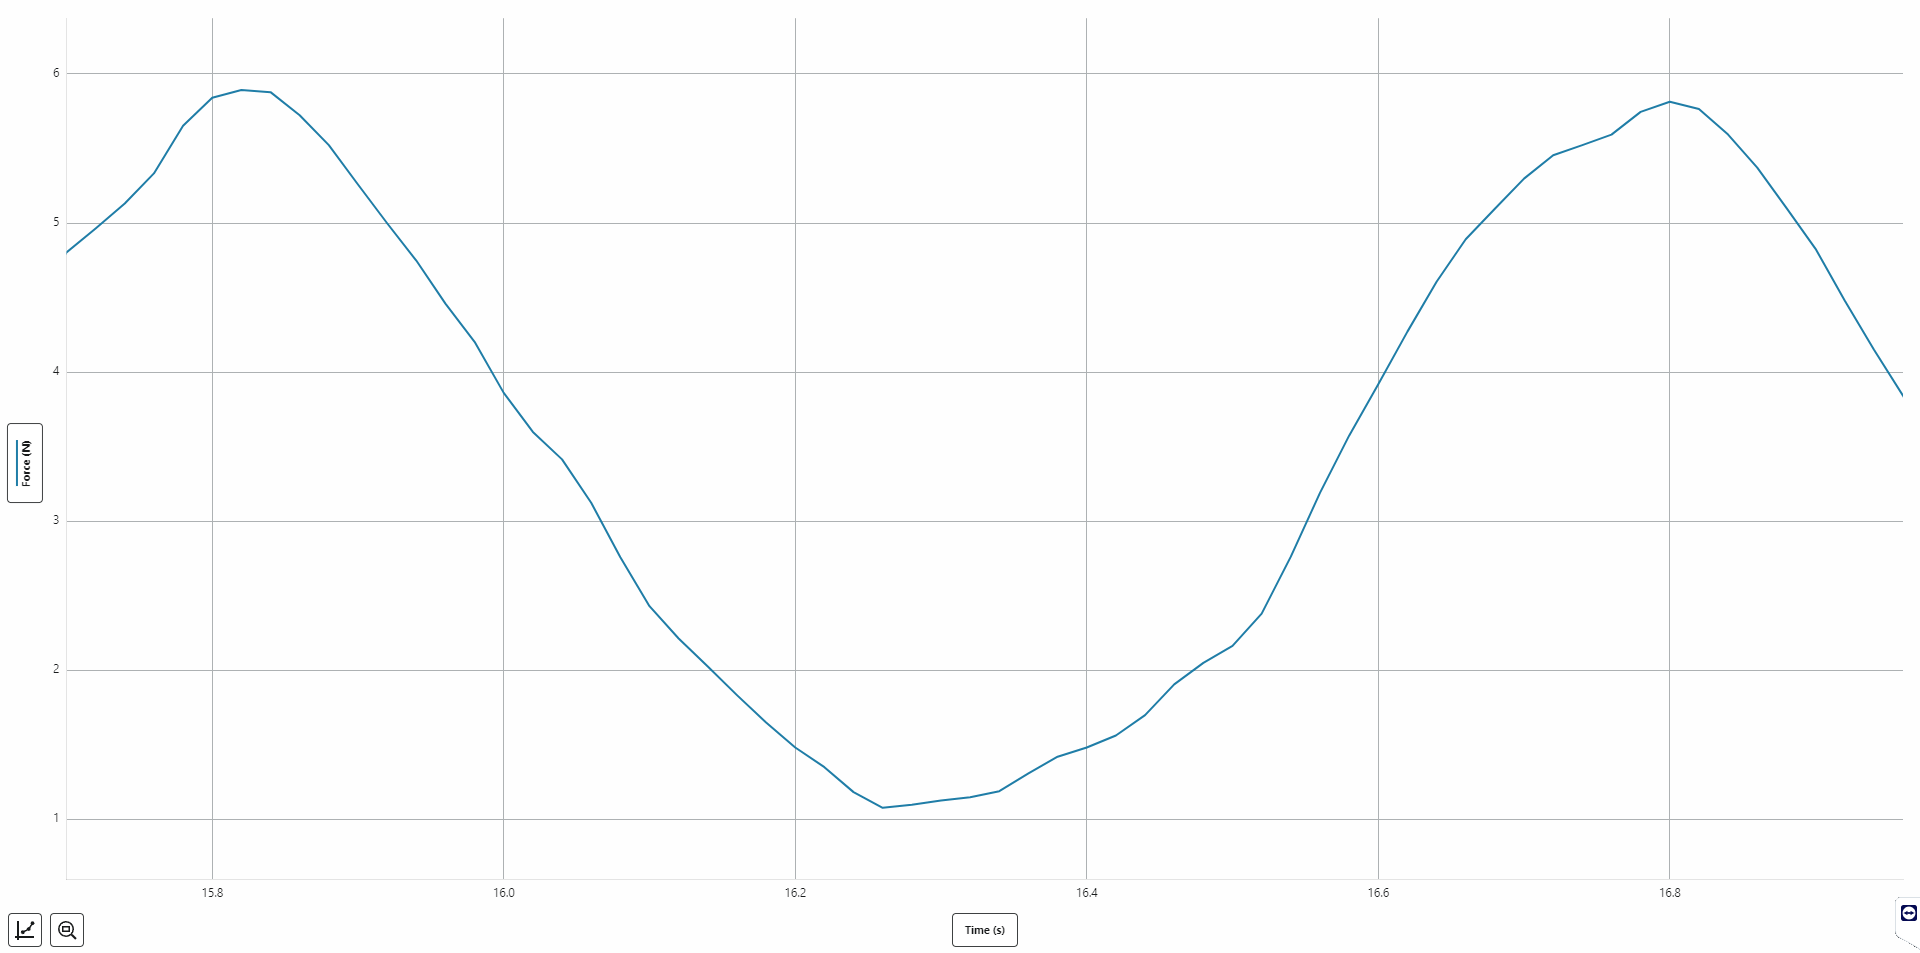
\includegraphics[width=0.8\textwidth]{Images/Loop the loop graph.png}};
			\draw[black, dashed] (-\HalfWidth,\TopLineY) -- (\HalfWidth,\TopLineY);
			\draw[black, dashed] (-\HalfWidth,\BottomLineY) -- (\HalfWidth,\BottomLineY);
			\filldraw[red!50!black] (BottomPos1) circle (.1) node[above=\TextGap, align=center] {Bottom of the vertical circle\\(15.82s, 5.89N)};
			\filldraw[green!50!black] (TopPos) circle (.1) node[above=\TextGap, align=center] {Top of the vertical circle\\(16.30s, 1.13N)};
			\filldraw[blue!50!black] (BottomPos2) circle (.1) node[above=\TextGap, align=center] {Bottom of the vertical circle\\(16.80s, 5.81N)};
		\end{tikzpicture}
		\caption{Graph of a complete vertical loop}
	\end{figure}
	At the bottom of the vertical circle, the tension force (emulating the lift force, $\vec{F_L}$) is greatest, which occurs at 15.82 seconds with 5.89N.\\
	Once the force meter (emulating motion of glider) reaches the top of the vertical circle, the tension force is at its least, which - when smoothing the curve of data and reducing random variation/noise - occurs at\\
	Check if sine model or quadratic helps - then return to this section.\\
	During the loop the loop, as the glider ascends, its kinetic energy ($E_K$) is converted into gravitational potential energy ($E_p$). As the glider descends, its gravitational potential energy ($E_p$) is converted back into kinetic energy ($E_K$).\\
	
	\subsection{Merit}
	\begin{align}
		E_K&=\frac{1}{2}m|\vec{v}|^2\\
		\therefore |\vec{v}|^2&\propto E_K\\
		|\vec{v}|&\propto \sqrt{E_K}
	\end{align}
	During the loop the loop, as the glider ascends, its kinetic energy ($E_K$) is converted into gravitational potential energy ($E_p$). This decreases its velocity as it is proportional to kinetic energy, which decreased when converted to gravitational potential energy. \\
	As the glider descends, its gravitational potential energy ($E_p$) is converted back into kinetic energy ($E_K$).This increases its velocity as it is proportional to kinetic energy, which increased when the gravitational potential energy was converted back into it.\\[\ParagraphSpacing]
	A glider's ability to successfully perform a vertical loop relies on its ability to provide an adequate lift force, increasing both net and centripetal force.
	\begin{align}
		|\vec{F_L}|&=\frac{1}{2}p|\vec{v}|^2AC_L \label{eq:lift}\\
		\therefore |\vec{F_L}|&\propto |\vec{v}|^2 \label{eq:lift-prop-vel} \\[\baselineskip]
		|\vec{F_{L_\text{top}}}|&=|\vec{F_c}|-|\vec{F_g}|\\
		|\vec{F_{L_\text{bottom}}}|&=|\vec{F_c}|+|\vec{F_g}|
	\end{align}
	\cref{eq:lift-prop-vel} shows that velocity is a major factor in the magnitude of the lift force. Without adequate velocity, inadequate lift force is provided for the vertical loop to be successful. As kinetic energy is converted to gravitational potential energy during ascent, if the velocity drops below what is required for the circular path radius its motion will instead imitate that of a projectile.\\
	Other factors proportional to velocity include surface area contacting air ($A$), and the coefficient of lift ($C_L$), determined by shape and angle of attack).\\
	Fluid density ($p$) is constant.\\[\ParagraphSpacing]
	During motion, 3 forces are acting on the stunt glider:
	\begin{enumerate}
		\item Gravity ($\vec{F_g}$) (i.e. Weight) always vertically downwards (i.e. toward center of Earth).
		\item Lift ($\vec{F_L}$) perpendicular to direction of velocity, toward the center of the circular path.
		\item Air Resistance ($\vec{F_R}$) (i.e. Friction, Drag) opposite to direction of velocity.
	\end{enumerate}
	Please note that vector arrow lengths are not perfectly proportionally accurate.
	\begin{center}
		\begin{tikzpicture}
			\pgfmathsetmacro{\MaxVelocityLength}{2}
			\pgfmathsetmacro{\MinVelocityLength}{1}
			\pgfmathsetmacro{\MaxResistanceLength}{\MaxVelocityLength*0.5}
			\pgfmathsetmacro{\MinResistanceLength}{\MinVelocityLength*0.5}
			\pgfmathsetmacro{\GravityLength}{1}
			\pgfmathsetmacro{\PathRadius}{5}
			\pgfmathsetmacro{\GliderPointRadius}{0.1}
			\coordinate(TopPos) at (0,\PathRadius);
			\coordinate(BottomPos) at (0,-\PathRadius);
			
			\draw[dashed, gray] (0,0) circle (\PathRadius);
			
			\filldraw[black] (TopPos) circle (\GliderPointRadius);
			\draw[->] (TopPos) -- ++(-\MinVelocityLength,0) node[left] {$\vec{v}$};
			\draw[->] (TopPos) -- ++(0,-\GravityLength) node[below] {$\vec{F_g}$};
			\draw[->] (TopPos) -- ++(0,-0.5) node[left] {$\vec{F_L}$};
			\draw[->] (TopPos) -- ++(\MinResistanceLength,0) node[right] {$\vec{F_R}$};
			
			\filldraw[black] (BottomPos) circle (\GliderPointRadius);
			\draw[->] (BottomPos) -- ++(\MaxVelocityLength,0) node[right] {$\vec{v}$};
			\draw[->] (BottomPos) -- ++(0,-\GravityLength) node[below] {$\vec{F_g}$};
			\draw[->] (BottomPos) -- ++(0,2) node[above] {$\vec{F_L}$};
			\draw[->] (BottomPos) -- ++(-\MaxResistanceLength,0) node[left] {$\vec{F_R}$};
		\end{tikzpicture}
	\end{center}
	\begin{figure}[H]
		\centering
		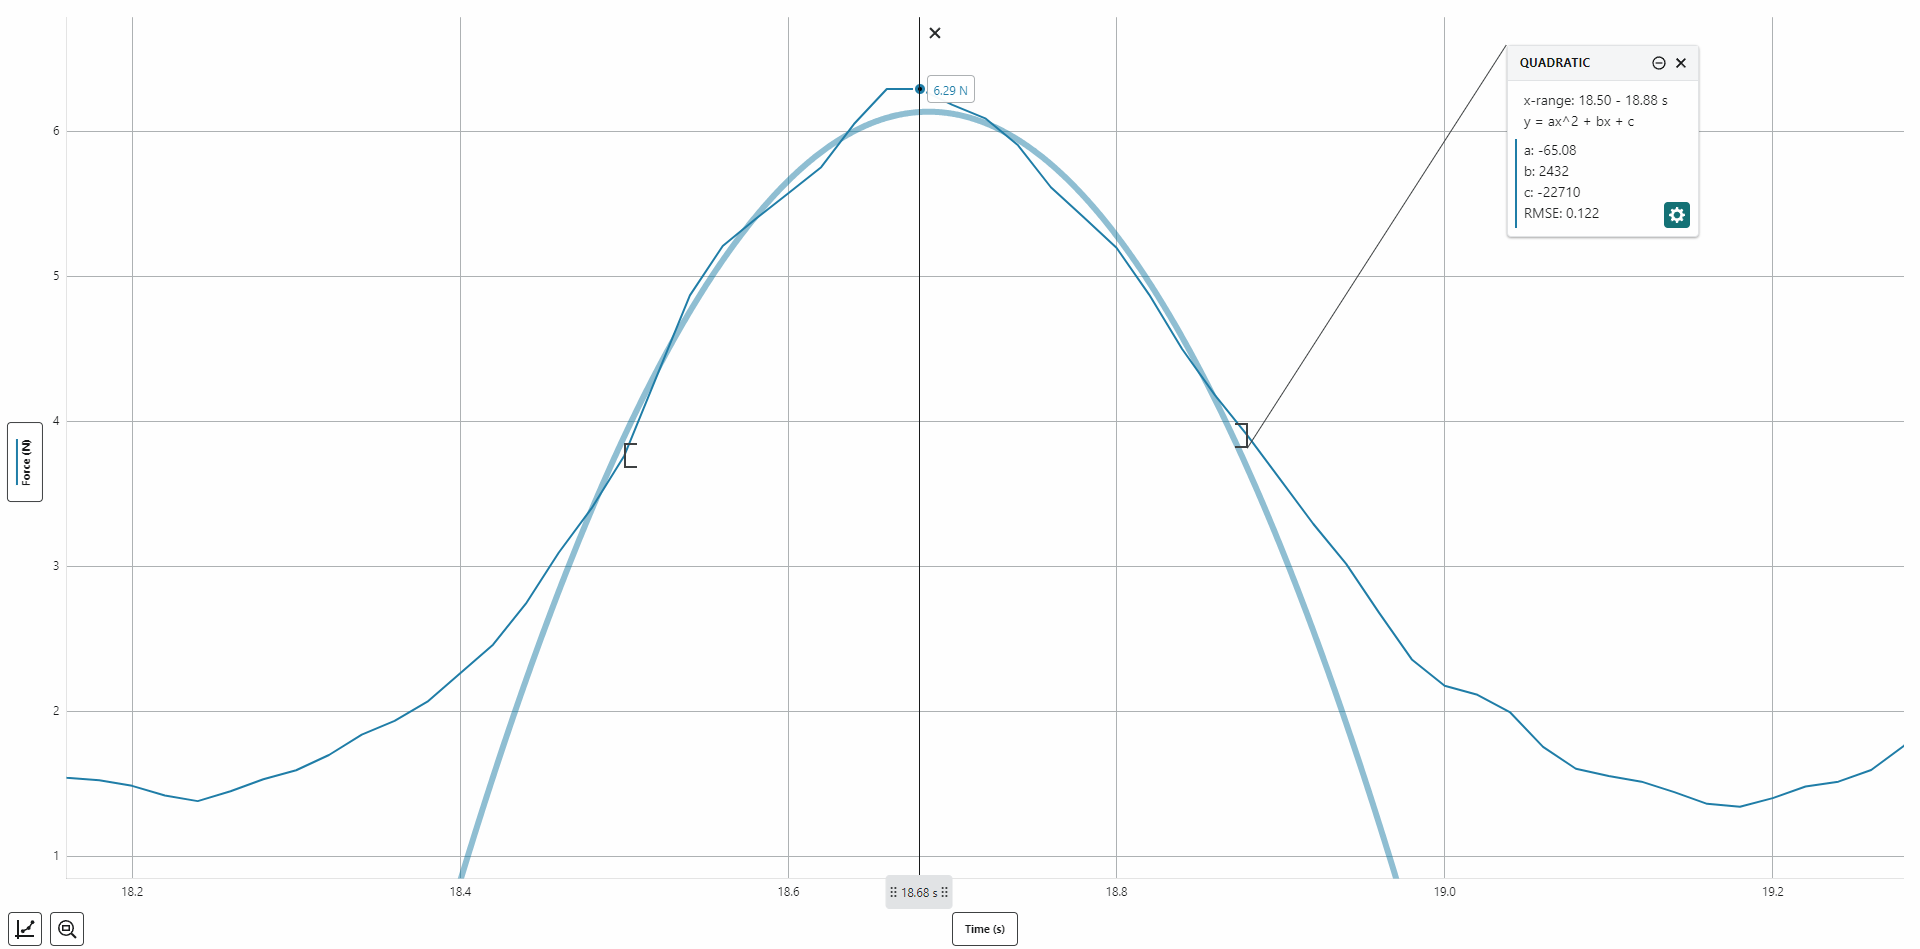
\includegraphics[width=0.8\textwidth]{Images/Dip in vertical circle.png}
		\caption{The dip section of vertical circular motion with a quadratic curve fit}
	\end{figure}
	Quadratic curve fit is applied to closely fit the lift force data in the section of the dip motion from 18.50s to 18.88s. It helps exclude random variation / noise in the data and provide consistent smoothness and symmetry. The line displayed in the center marks 18.68s, which is when the emulated glider reaches its lowest vertical height (i.e. lowest point in the dip), also aligning with the local peak in the emulated lift force at 6.29N. The reason for the greatest lift force being required at the bottom of the loop the loop is due to its direction oppositely opposing gravity, requiring the greatest magnitude to provide sufficient centripetal force for the vertical loop's radius. The velocity is also greatest here as it has the greatest $E_K:E_P$ ratio (i.e. $\frac{E_K}{E_P}$ is at its greatest in the time series) (as previously explained) which is a major factor in causing that required greatest lift force (as explained in previous equations) $\because E_K\propto|\vec{v}|^2\propto |\vec{F_L}|$).
	\subsection{Excellence}
	\begin{center}
		\begin{tikzpicture}
			\pgfmathsetmacro{\SqrtTwo}{1.414213562}
			\pgfmathsetmacro{\ARVel}{0.3}
			\pgfmathsetmacro{\VelA}{2}
			\pgfmathsetmacro{\VelB}{1.75}
			\pgfmathsetmacro{\VelC}{1.5}
			\pgfmathsetmacro{\VelD}{1.25}
			\pgfmathsetmacro{\VelE}{1}
			\pgfmathsetmacro{\LA}{2.1}
			\pgfmathsetmacro{\LB}{1.7}
			\pgfmathsetmacro{\LC}{1.3}
			\pgfmathsetmacro{\LD}{0.9}
			\pgfmathsetmacro{\LE}{0.5}
			\pgfmathsetmacro{\GravityLength}{1}
			\pgfmathsetmacro{\PathRadius}{9}
			\pgfmathsetmacro{\DiagCoord}{\PathRadius/\SqrtTwo}
			\pgfmathsetmacro{\GliderPointRadius}{0.1}
			\coordinate(TopPos) at (0,\PathRadius);
			\coordinate(RightPos) at (\PathRadius, 0);
			\coordinate(LeftPos) at (-\PathRadius, 0);
			\coordinate(BottomPos) at (0,-\PathRadius);
			\coordinate(URPos) at (\DiagCoord, \DiagCoord);
			\coordinate(LRPos) at (\DiagCoord, -\DiagCoord);
			\coordinate(ULPos) at (-\DiagCoord, \DiagCoord);
			\coordinate(LLPos) at (-\DiagCoord, -\DiagCoord);
			
			\draw[dashed, gray] (0,0) circle (\PathRadius);
			
			% TOP
			\filldraw[black] (TopPos) circle (\GliderPointRadius);
			\draw[->] (TopPos) -- ++(-\VelE,0) node[left] {$\vec{v}$};
			\draw[->] (TopPos) -- ++(0,-\GravityLength) node[below] {$\vec{F_g}$};
			\draw[->] (TopPos) -- ++(0,-\LE) node[left] {$\vec{F_L}$};
			\draw[->] (TopPos) -- ++(\VelE*\ARVel,0) node[right] {$\vec{F_R}$};
			
			% BOTTOM
			\filldraw[black] (BottomPos) circle (\GliderPointRadius);
			\draw[->] (BottomPos) -- ++(\VelA,0) node[right] {$\vec{v}$};
			\draw[->] (BottomPos) -- ++(0,-\GravityLength) node[below] {$\vec{F_g}$};
			\draw[->] (BottomPos) -- ++(0,\LA) node[above] {$\vec{F_L}$};
			\draw[->] (BottomPos) -- ++(-\VelA*\ARVel,0) node[left] {$\vec{F_R}$};
			
			% RIGHT
			\filldraw[black] (RightPos) circle (\GliderPointRadius);
			\draw[->] (RightPos) -- ++(0, \VelC) node[above] {$\vec{v}$};
			\draw[->] (RightPos) -- ++(0,-\GravityLength) node[below] {$\vec{F_g}$};
			\draw[->] (RightPos) -- ++(-\LC,0) node[left] {$\vec{F_L}$};
			\draw[->] (RightPos) -- ++(0,-\VelC*\ARVel) node[right] {$\vec{F_R}$};
			
			% LEFT
			\filldraw[black] (LeftPos) circle (\GliderPointRadius);
			\draw[->] (LeftPos) -- ++(0, -\VelC) node[below] {$\vec{v}$};
			\draw[->] (LeftPos) -- ++(0,-\GravityLength) node[right] {$\vec{F_g}$};
			\draw[->] (LeftPos) -- ++(\LC,0) node[right] {$\vec{F_L}$};
			\draw[->] (LeftPos) -- ++(0,\VelC*\ARVel) node[above] {$\vec{F_R}$};
			
			% LOWER RIGHT
			\filldraw[black] (LRPos) circle (\GliderPointRadius);
			\draw[->] (LRPos) -- ++(\VelB/\SqrtTwo, \VelB/\SqrtTwo) node[above right] {$\vec{v}$};
			\draw[->] (LRPos) -- ++(0,-\GravityLength) node[below] {$\vec{F_g}$};
			\draw[->] (LRPos) -- ++(-\LB/\SqrtTwo,\LB/\SqrtTwo) node[above left] {$\vec{F_L}$};
			\draw[->] (LRPos) -- ++(-\VelB/\SqrtTwo*\ARVel,-\VelB/\SqrtTwo*\ARVel) node[below left] {$\vec{F_R}$};
			
			% LOWER LEFT
			\filldraw[black] (LLPos) circle (\GliderPointRadius);
			\draw[->] (LLPos) -- ++(\VelB/\SqrtTwo, -\VelB/\SqrtTwo) node[below right] {$\vec{v}$};
			\draw[->] (LLPos) -- ++(0,-\GravityLength) node[below] {$\vec{F_g}$};
			\draw[->] (LLPos) -- ++(\LB/\SqrtTwo,\LB/\SqrtTwo) node[above right] {$\vec{F_L}$};
			\draw[->] (LLPos) -- ++(-\VelB/\SqrtTwo*\ARVel,\VelB/\SqrtTwo*\ARVel) node[above left] {$\vec{F_R}$};
			
			% UPPER RIGHT
			\filldraw[black] (URPos) circle (\GliderPointRadius);
			\draw[->] (URPos) -- ++(-\VelD/\SqrtTwo, \VelD/\SqrtTwo) node[above left] {$\vec{v}$};
			\draw[->] (URPos) -- ++(0,-\GravityLength) node[below] {$\vec{F_g}$};
			\draw[->] (URPos) -- ++(-\LD/\SqrtTwo,-\LD/\SqrtTwo) node[below left] {$\vec{F_L}$};
			\draw[->] (URPos) -- ++(\VelD/\SqrtTwo*\ARVel,-\VelD/\SqrtTwo*\ARVel) node[below right] {$\vec{F_R}$};
			
			% UPPER LEFT
			\filldraw[black] (ULPos) circle (\GliderPointRadius);
			\draw[->] (ULPos) -- ++(-\VelD/\SqrtTwo, -\VelD/\SqrtTwo) node[below left] {$\vec{v}$};
			\draw[->] (ULPos) -- ++(0,-\GravityLength) node[below] {$\vec{F_g}$};
			\draw[->] (ULPos) -- ++(\LD/\SqrtTwo,-\LD/\SqrtTwo) node[below right] {$\vec{F_L}$};
			\draw[->] (ULPos) -- ++(\VelD/\SqrtTwo*\ARVel,\VelD/\SqrtTwo*\ARVel) node[above right] {$\vec{F_R}$};
			
			% INFO
			\pgfmathsetmacro{\InfoSpacing}{15}
			\node at (0,0) [align=center] {$\vec{F_g}$ Gravity\\[\InfoSpacing]$\vec{F_L}$ Lift\\[\InfoSpacing]$\vec{F_R}$ Air Resistance\\[\InfoSpacing]$\vec{v}$ Velocity};
		\end{tikzpicture}
	\end{center}
	\begin{table}[H]
		\renewcommand{\arraystretch}{1.5}
		\begin{tabularx}{\textwidth}{|>{\raggedright\arraybackslash}X|||>{\raggedright\arraybackslash}X|}
			\hline
			Bottom of loop ($\vec{v}$ direction is horizontally right)
			&
			Top of loop ($\vec{v}$ direction is horizontally left)\\
			\hline
			\begin{center}
				\begin{tikzpicture}
					\pgfmathsetmacro{\LA}{2.1}
					\pgfmathsetmacro{\VelA}{2}
					\pgfmathsetmacro{\GravityLength}{1}
					\pgfmathsetmacro{\GliderPointRadius}{0.1}
					\pgfmathsetmacro{\ARVel}{0.3}
					\pgfmathsetmacro{\FC}{\LA-\GravityLength}
					% BOTTOM
					\draw[->, red!50!white, line width=1mm] (0,0) -- ++(0,\FC) node[right,xshift=1mm] {$\vec{F_c}$};
					\draw[->] (0,0) -- ++(\VelA,0) node[right] {$\vec{v}$};
					\draw[->] (0,0) -- ++(0,-\GravityLength) node[below] {$\vec{F_g}$};
					\draw[->] (0,0) -- ++(0,\LA) node[above] {$\vec{F_L}$};
					\draw[->] (0,0) -- ++(-\VelA*\ARVel,0) node[left] {$\vec{F_R}$};
					\filldraw[black] (0,0) circle (\GliderPointRadius);
				\end{tikzpicture}
			\end{center}
			&
			\begin{center}
				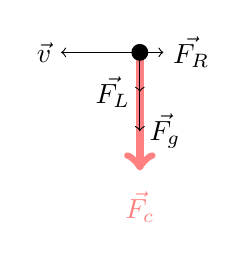
\begin{tikzpicture}
					\pgfmathsetmacro{\LE}{0.5}
					\pgfmathsetmacro{\VelE}{1}
					\pgfmathsetmacro{\GravityLength}{1}
					\pgfmathsetmacro{\GliderPointRadius}{0.1}
					\pgfmathsetmacro{\ARVel}{0.3}
					\pgfmathsetmacro{\FC}{\LE+\GravityLength}
					% TOP
					\draw[->, red!50!white, line width=1mm] (0,0) -- ++(0,-\FC) node[below,yshift=-1mm] {$\vec{F_c}$};
					\filldraw[black] (0,0) circle (\GliderPointRadius);
					\draw[->] (0,0) -- ++(-\VelE,0) node[left] {$\vec{v}$};
					\draw[->] (0,0) -- ++(0,-\GravityLength) node[right] {$\vec{F_g}$};
					\draw[->] (0,0) -- ++(0,-\LE) node[left] {$\vec{F_L}$};
					\draw[->] (0,0) -- ++(\VelE*\ARVel,0) node[right] {$\vec{F_R}$};
				\end{tikzpicture}
			\end{center}\\
			\hline
			\parbox{0.45\textwidth}{
				\begin{align}
					\vec{F_c} &= \vec{F_L} + \vec{F_g} \\
					|\vec{F_c}| &= |\vec{F_L}| - |\vec{F_g}|
				\end{align}
			}
			&
			\parbox{0.45\textwidth}{
				\begin{align}
					\vec{F_c} &= \vec{F_L} + \vec{F_g} \\
					|\vec{F_c}| &= |\vec{F_L}| + |\vec{F_g}|
				\end{align}
			}\\
			\hline
			Lift and gravity force vectors add. Gravity reduces magnitude of centripetal force as it opposes in direction.
			&
			Lift and gravity force vectors add. Gravity increases magnitude of centripetal force as it aligns in direction.\\
			\hline
			On the graph from our force meter model, this position has the greatest tension force, which is used to emulate the lift force of the glider. As previously explained, this is what we should expect as kinetic energy, velocity, and consequently the lift force of glider should be greatest, which is crucial for it to counter gravity and provide sufficient magnitude.
			
			\vspace{\baselineskip}
			Although the tension force doesn't perfectly act as a lift force in that its force isn't proportional to velocity in the same way it instead almost instantaneously provides adequate force to decelerate outwards velocity to zero and if it remains on the circumference of the path with force applied against it, tension provides greater than or equal to to counter it.
			&
			On the graph from our force meter mode, this position has the least tension force which is used to emualte the lift force of the glider. As explained, this is what we should expect as kinetic energy, velocity and consequently the lift force of the glider should be least - instead the force of gravity typically contributes the majority towards the centripetal force, with the downwards lift force contributing a minority to its magnitude.\\
			\hline
		\end{tabularx}
	\end{table}
	
	\begin{table}[H]
		\renewcommand{\arraystretch}{1.5}
		\begin{tabularx}{\textwidth}{|>{\raggedright\arraybackslash}X|||>{\raggedright\arraybackslash}X|}
			\hline
			Right of loop ($\vec{v}$ direction is vertically upwards)
			&
			Bottom Right of loop ($\vec{v}$ direction is right at $45^\circ$ above horizontal)\\
			\hline
			\begin{center}
				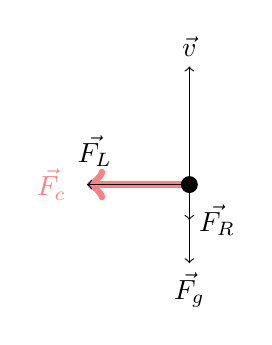
\begin{tikzpicture}
					\pgfmathsetmacro{\LC}{1.3}
					\pgfmathsetmacro{\VelC}{1.5}
					\pgfmathsetmacro{\GravityLength}{1}
					\pgfmathsetmacro{\GliderPointRadius}{0.1}
					\pgfmathsetmacro{\ARVel}{0.3}
					% RIGHT
					\draw[->, red!50!white, line width=1mm] (0,0) -- ++(-\LC,0) node[left,xshift=-1mm] {$\vec{F_c}$};
					\filldraw[black] (0,0) circle (\GliderPointRadius);
					\draw[->] (0,0) -- ++(0, \VelC) node[above] {$\vec{v}$};
					\draw[->] (0,0) -- ++(0,-\GravityLength) node[below] {$\vec{F_g}$};
					\draw[->] (0,0) -- ++(-\LC,0) node[above,xshift=1mm,yshift=1mm] {$\vec{F_L}$};
					\draw[->] (0,0) -- ++(0,-\VelC*\ARVel) node[right] {$\vec{F_R}$};
				\end{tikzpicture}
			\end{center}
			&
			\begin{center}
				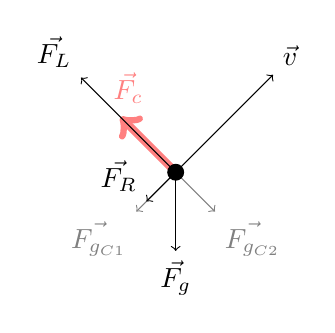
\begin{tikzpicture}
					\pgfmathsetmacro{\SqrtTwo}{1.414213562}
					\pgfmathsetmacro{\VelB}{1.75}
					\pgfmathsetmacro{\LB}{1.7}
					\pgfmathsetmacro{\GravityLength}{1}
					\pgfmathsetmacro{\GravityComponent}{\GravityLength/\SqrtTwo}
					\pgfmathsetmacro{\GliderPointRadius}{0.1}
					\pgfmathsetmacro{\ARVel}{0.3}
					\pgfmathsetmacro{\FC}{\LB-\GravityComponent}
					% LOWER RIGHT
					\draw[->, red!50!white, line width=1mm] (0,0) -- ++(-\FC/\SqrtTwo,\FC/\SqrtTwo) node[above,xshift=1mm] {$\vec{F_c}$};
					\draw[->] (0,0) -- ++(\VelB/\SqrtTwo, \VelB/\SqrtTwo) node[above right] {$\vec{v}$};
					\draw[->] (0,0) -- ++(0,-\GravityLength) node[below] {$\vec{F_g}$};
					\draw[->] (0,0) -- ++(-\LB/\SqrtTwo,\LB/\SqrtTwo) node[above left] {$\vec{F_L}$};
					\draw[->, gray] (0,0) -- ++(-\GravityComponent/\SqrtTwo,-\GravityComponent/\SqrtTwo) node[below left] {$\vec{F_{g_{C1}}}$};
					\draw[->, gray] (0,0) -- ++(\GravityComponent/\SqrtTwo,-\GravityComponent/\SqrtTwo) node[below right] {$\vec{F_{g_{C2}}}$};
					\draw[->] (0,0) -- ++(-\VelB/\SqrtTwo*\ARVel,-\VelB/\SqrtTwo*\ARVel) node[above left] {$\vec{F_R}$};
					\filldraw[black] (0,0) circle (\GliderPointRadius);
				\end{tikzpicture}
			\end{center}\\
			\hline
			\parbox{0.45\textwidth}{
				\begin{align}
					\vec{F_c} &= \vec{F_L} \\
					|\vec{F_c}| &= |\vec{F_L}|
				\end{align}
			}
			&
			\parbox{0.45\textwidth}{
				\vspace{10pt}
				$\vec{F_{g_{C1}}}$ is left at $45^\circ$ below horizontal \\
				$\vec{F_{g_{C2}}}$ is right at $45^\circ$ below horizontal
				\begin{align}
					|\vec{F_{g_{C2}}}| &= |\vec{F_{g_{C1}}}| \\
					&= |\vec{F_g}| \times \sin (45^\circ) \\
					&= |\vec{F_g}| \times \frac{\sqrt{2}}{2} \\
					&= \frac{|\vec{F_g}|\sqrt{2}}{2} \\[20pt]
					\vec{F_c} &= \vec{F_L} + \vec{F_{g_{C2}}} \\
					|\vec{F_c}| &= |\vec{F_L}| - |\vec{F_{g_{C2}}}| \\
					&= |\vec{F_L}| - \frac{|\vec{F_g}|\sqrt{2}}{2}
				\end{align}
			}\\
			\hline
			Centripetal force can only be provided by lift force. All other forces are vertical (have no horizontal component that can contribute to centripetal force).
			&
			Lift and only a component of gravity ($\vec{F_{g_{C2}}}$) add to provide the centripetal force. That component of gravity contributes in decreasing the magnitude of centripetal force as it opposes in direction.\\
			\hline
			On the graph, We can expect this position of the loop to have a tension force exactly halfway in between the peak and trough. The difference in velocity between top and bottom will determine how much the tension force varies throughout the loop.
			
			\vspace{\baselineskip}
			If proportionally significant, we can expect proportionally significant change in tension/lift, else if very little proportional change we can expect very little proportional difference to the lift (and centripetal since they're the same, solely provided by lift) force.
			
			\vspace{\baselineskip}
			By this point it has gained half the gravitation potential energy that it will in total, and hence lost exactly half of the kinetic energy it will lose in total. So velocity is exactly half that change and consequently lift force is exactly half.
			
			\vspace{\baselineskip}
			REWORD AND PROVIDE EQUATION PROOF?
			&
			On the graph, we can expect this position of the loop to have a tension force exactly a quarter of the range above the minimum of the range. \\
			\hline
		\end{tabularx}
	\end{table}
	
	%Using the force meter model, take measurements of the motion to calculate the force at the bottom of the loop when the model glider moves with the minimum velocity that still allows the model of the glider to complete a full loop.
	%Compare the value of force calculated with the actual measured value and explain any differences by considering accuracy in the measurements.
	
	I'll assume that at the top of the loop, the downwards lift force is zero. In reality, this would never happen. Unless its velocity was perfectly zero (completely stationary), \cref{eq:lift} and \cref{eq:lift-prop-vel} prove there must also be a lift force. Depending on the velocity (ranging from minimum to excessive), that lift force could range from negligible to decently large.\\
	\cref{eq:min-vel} represents the minimum velocity $|\vec{v}|$ required to produce adequate centripetal acceleration $|\vec{a_c}|$ for a circular path with radius $r$.
	\begin{align}
		|\vec{a_c}|&=\frac{|\vec{v}|^2}{r}\\
		|\vec{v_{\text{top}}}|&=\sqrt{|\vec{a_c}|r} \label{eq:min-vel}\\
		&=\sqrt{(9.81)\left(\frac{96.4}{100}\right)}\\
		&= \SI{3.08}{\meter\per\second} \quad (2\, \text{d.p.})
	\end{align}
	The following equations solve for the "lift" (emulated by tension) force at the bottom of the modeled vertical loop with tension force.
	\begin{align}
		E_{K_{\text{top}}}&=\frac{1}{2}m|\vec{v_{\text{top}}}|^2\\
		&=\frac{1}{2}\left(\frac{89.4}{1000}\right)(3.08)^2\\
		&=\SI{0.42}{\joule} \quad (2\, \text{d.p.})\\[\baselineskip]
		\Delta h&=h_{\text{top}}-h_{\text{bottom}}\\
		&\approx2r\\
		%\text{\tiny (Approximate as our hand is the pivot which can't be kept flawlessly stationary.)}\\[\baselineskip]
		\Delta E_p&=mg\Delta h\\
		&\approx mg2r\\[\baselineskip]
		E_{K_{\text{bottom}}}&=E_{K_{\text{top}}}+\Delta E_p\\
		&=\frac{1}{2}m|\vec{v_{\text{top}}}|^2+mg\Delta h\\
		&\approx \frac{1}{2}m|\vec{v_{\text{top}}}|^2+mg2r\\
		&\approx \frac{1}{2}\left(\frac{89.4}{1000}\right)(3.08)^2 + \left(\frac{89.4}{1000}\right)(9.81)\left(\frac{2\times96.4}{100}\right)\\
		&\approx \SI{2.11}{\joule} \quad (2\, \text{d.p.})\\[\baselineskip]
		|\vec{v_{\text{bottom}}}|&=\sqrt{\frac{2E_{K_{\text{bottom}}}}{m}}\\
		&\approx \sqrt{\frac{2(2.11)}{\left(\dfrac{89.4}{1000}\right)}}\\
		&\approx \SI{6.88}{\meter\per\second} \quad (2\, \text{d.p.})\\[\baselineskip]
		|\vec{F_{c_{\text{bottom}}}}|&=\frac{m|\vec{v_{\text{bottom}}}|^2}{r}\\
		&\approx\frac{\left(\dfrac{89.4}{1000}\right)(6.88)^2}{\left(\dfrac{96.4}{100}
			\right)}\\
		&\approx \SI{4.39}{\newton} \quad (2\, \text{d.p.})\\[\baselineskip]
		|\vec{F_{L_\text{bottom}}}|-|\vec{F_g}|&=|\vec{F_{c_\text{bottom}}}|\\
		|\vec{F_{L_{\text{bottom}}}}|&=|\vec{F_{c_{\text{bottom}}}}|+|\vec{F_g}|\\
		&=|\vec{F_{c_{\text{bottom}}}}|+m|\vec{g}|\\
		&\approx(4.39)+\left(\frac{89.4}{1000}\right)(9.81)\\
		&\approx \SI{5.27}{\newton} \quad (2\, \text{d.p.})
	\end{align}
	
	\begin{figure}[H]
		\centering
		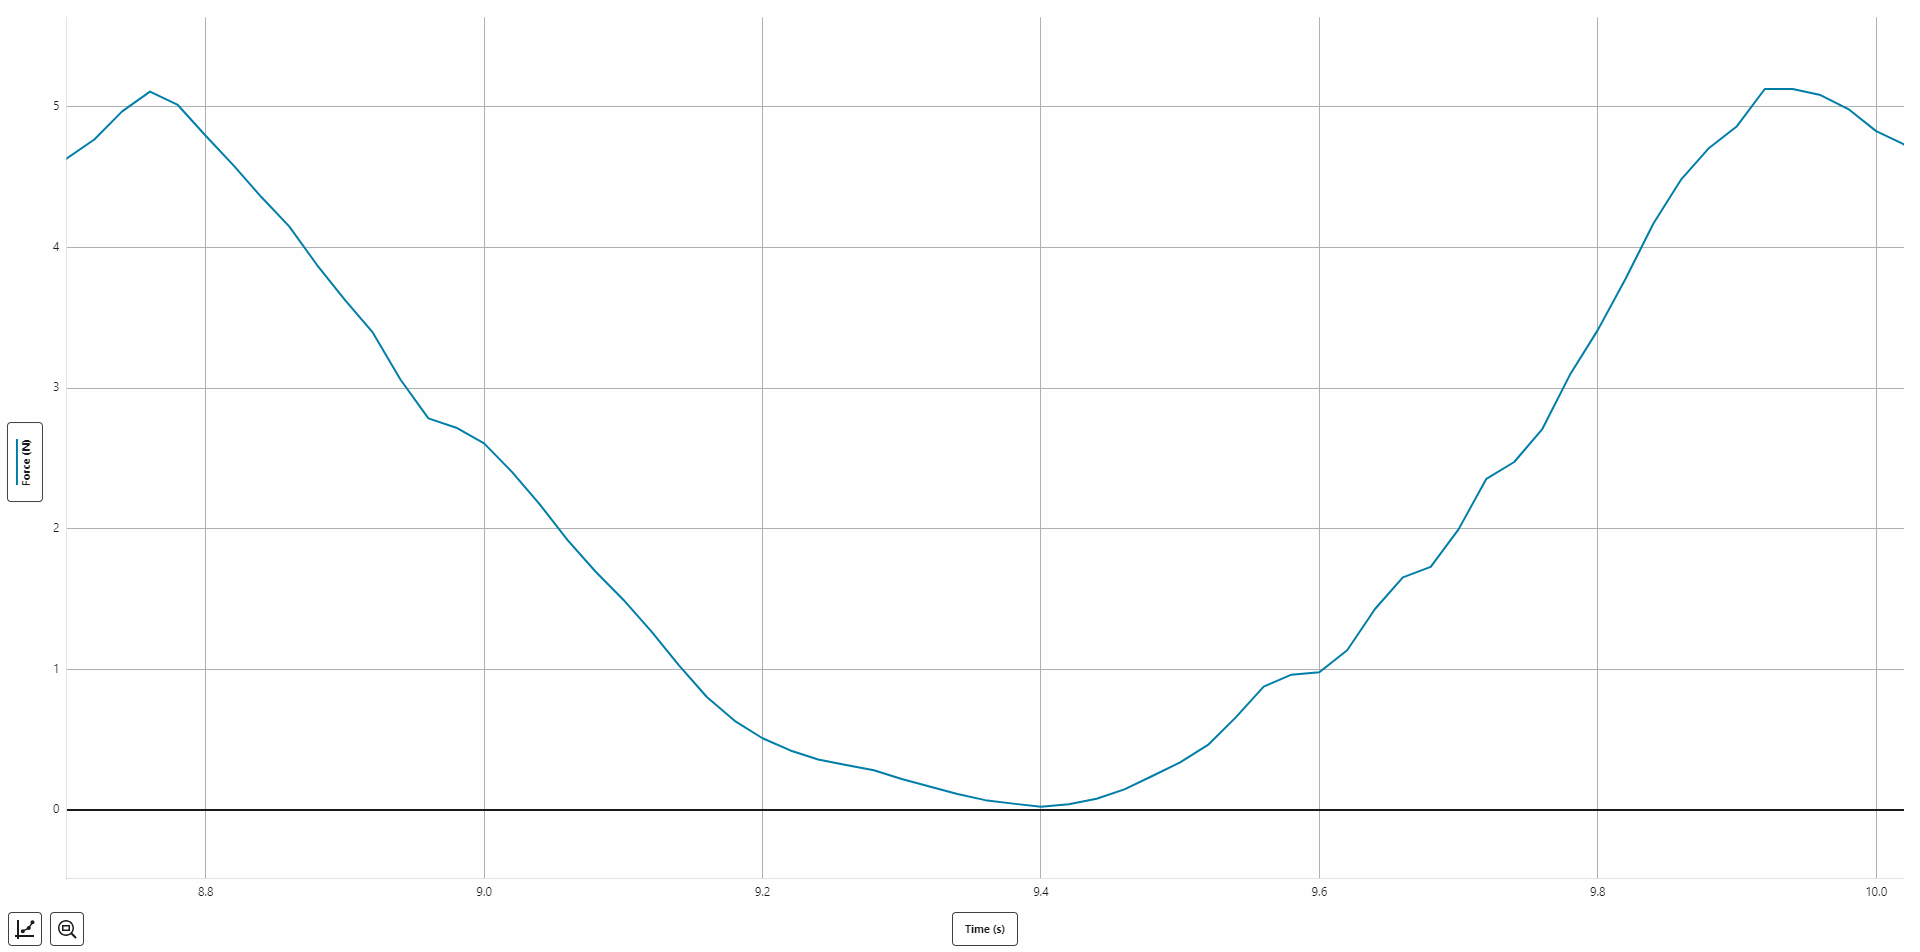
\includegraphics[width=0.8\textwidth]{Images/Tension at Bottom}
		\caption{Tension force in string during vertical loop}
	\end{figure}
	In the data, we can see that at the bottom of the vertical loop (i.e. at the peaks of the graph) it has $F_{T_\text{bottom}}\approx \SI{5.12}{\newton} \quad (2\, \text{d.p.})$. This is marginally less than the calculated value, which is expected as air resistance is not taken into account in the calculations. In a real world scenario, the air resistance causes a minor proportion of the kinetic energy to convert into other forms, such as thermal energy (heat) and sound energy. That reduction in kinetic energy causes less velocity magnitude, which would cause less lift force at the bottom due to eqXXX or in the model, less tension force as XGUYWGFUYGWA
	
	\section{Banked Corner}
	\subsection{Diagrams}
	Note: Air resistance and velocity have been omitted from the following diagrams. Velocity is always tangent to the circular path. Air resistance is always opposite in direction to velocity. Their magnitudes will correlate in that $|\vec{F_R}| \propto |\vec{v}|^2$.\\
	\vspace{\baselineskip}
		\begin{center}
		\begin{tikzpicture}
			\pgfmathsetmacro{\GravityLength}{1}
			\pgfmathsetmacro{\GliderPointRadius}{0.1}
			\pgfmathsetmacro{\CircularPathRadius}{5}
			\coordinate (GliderPoint) at (-\CircularPathRadius,0);
			\coordinate (PivotPoint) at (0,\CircularPathRadius);
			\coordinate (CenterPoint) at (0,0);
			\draw [gray, dotted] (-\CircularPathRadius,0) -- (PivotPoint);
			\draw [gray, dotted] (\CircularPathRadius,0) -- (PivotPoint);
			\draw [lightgray, dotted] (CenterPoint) -- (PivotPoint);
			\draw [lightgray, dotted] (GliderPoint) -- (\CircularPathRadius,0);
			\draw[gray, dashed] (CenterPoint) ellipse (5 and 1);
			\draw [->] (-\CircularPathRadius,0) -- ++(0, -\GravityLength) node[below] {$\vec{F_g}$};
			\draw[draw=none, postaction={decorate}] (0,0) -- ++(0, -\GravityLength);
			\draw [->] (-\CircularPathRadius,0) -- ++(\GravityLength, \GravityLength) node[above right] {$\vec{F_L}$};
			\draw[draw=none, gray, postaction={decorate}] (0,0) -- ++(0, \GravityLength);
			\filldraw[black] (GliderPoint) circle (\GliderPointRadius);
			\pic [draw, "$\theta$", angle radius=1cm, angle eccentricity=1.5] {angle = GliderPoint--PivotPoint--CenterPoint};
		\end{tikzpicture}
	\end{center}
	
	\begin{table}[H]
		\renewcommand{\arraystretch}{1.5}
		\begin{tabularx}{\textwidth}{X|X}
			Components:
			&
			Vector Addition:\\
			\hline
			\vspace{\baselineskip}
			\begin{tikzpicture}[
				% Define the decoration for double congruence marks
				decoration={
					markings,
					mark=at position 0.5 with {
						\draw[thick] (-2pt, -4pt) -- (-2pt, 4pt);
						\draw[thick] (2pt, -4pt) -- (2pt, 4pt);
					}
				}
				]
				\pgfmathsetmacro{\GravityLength}{3}
				\pgfmathsetmacro{\GliderPointRadius}{0.1}
				\draw [->] (0,0) -- ++(0, -\GravityLength) node[below] {$\vec{F_g}$};
				\draw[draw=none, postaction={decorate}] (0,0) -- ++(0, -\GravityLength);
				\draw [->] (0,0) -- ++(\GravityLength, \GravityLength) node[above right] {$\vec{F_L}$};
				\draw [->, gray, dashed] (0,0) -- ++(\GravityLength, 0) node[right] {$\vec{F_{L_x}}$};
				\draw [->, gray, dashed] (0,0) -- ++(0, \GravityLength) node[above] {$\vec{F_{L_y}}$};
				\draw[draw=none, gray, postaction={decorate}] (0,0) -- ++(0, \GravityLength);
				\filldraw[black] (0,0) circle (\GliderPointRadius);
				\coordinate (GliderPoint) at (0,0);
				\coordinate (LiftPoint) at (\GravityLength,\GravityLength);
				\coordinate (LiftXPoint) at (\GravityLength,0);
				\coordinate (LiftYPoint) at (0,\GravityLength);
				\pic [draw, "$\theta$", angle radius=0.8cm, angle eccentricity=1.5] {angle = GliderPoint--LiftPoint--LiftXPoint};
				\draw [lightgray, dotted] (LiftPoint)--(LiftXPoint);
				\draw [lightgray, dotted] (LiftPoint)--(LiftYPoint);
			\end{tikzpicture}
			&
			\vspace{\baselineskip}
			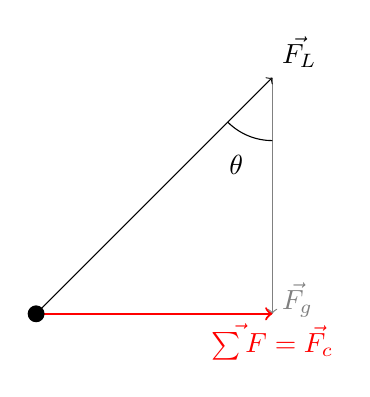
\begin{tikzpicture}[
				% Define the decoration for double congruence marks
				decoration={
					markings,
					mark=at position 0.5 with {
						\draw[thick] (-2pt, -4pt) -- (-2pt, 4pt);
						\draw[thick] (2pt, -4pt) -- (2pt, 4pt);
					}
				}
				]
				\pgfmathsetmacro{\GravityLength}{3}
				\pgfmathsetmacro{\GliderPointRadius}{0.1}
				\draw [->, gray] (\GravityLength, \GravityLength) -- ++(0, -\GravityLength) node[right, yshift=5pt] {$\vec{F_g}$};
				\draw [->] (0,0) -- ++(\GravityLength, \GravityLength) node[above right] {$\vec{F_L}$};
				\draw [->, red, thick] (0,0) -- ++(\GravityLength, 0) node[below] {$\vec{\sum F}=\vec{F_c}$};
				\filldraw[black] (0,0) circle (\GliderPointRadius);
				\coordinate (GliderPoint) at (0,0);
				\coordinate (LiftPoint) at (\GravityLength,\GravityLength);
				\coordinate (LiftXPoint) at (\GravityLength,0);
				\pic [draw, "$\theta$", angle radius=0.8cm, angle eccentricity=1.5] {angle = GliderPoint--LiftPoint--LiftXPoint};
			\end{tikzpicture}\\
			\begin{tikzpicture}[
				% Define the decoration for double congruence marks
				decoration={
					markings,
					mark=at position 0.5 with {
						\draw[thick] (-2pt, -4pt) -- (-2pt, 4pt);
						\draw[thick] (2pt, -4pt) -- (2pt, 4pt);
					}
				}
				]
				\pgfmathsetmacro{\GravityLength}{3}
				\pgfmathsetmacro{\GliderPointRadius}{0.1}
				\draw [->, lightgray] (0,0) -- ++(0, -\GravityLength) node[below] {$\vec{F_g}$};
				\draw[draw=none, lightgray, postaction={decorate}] (0,0) -- ++(0, -\GravityLength);
				\draw [->, lightgray] (0,0) -- ++(\GravityLength, \GravityLength) node[above right] {$\vec{F_L}$};
				\draw [->, red, thick] (0,0) -- ++(\GravityLength, 0) node[right] {$\vec{F_{L_x}}=\vec{\sum F}=\vec{F_c}$};
				\draw [->, lightgray, dashed] (0,0) -- ++(0, \GravityLength) node[above] {$\vec{F_{L_y}}$};
				\draw[draw=none, lightgray, postaction={decorate}] (0,0) -- ++(0, \GravityLength);
				\filldraw[black] (0,0) circle (\GliderPointRadius);
				\coordinate (GliderPoint) at (0,0);
				\coordinate (LiftPoint) at (\GravityLength,\GravityLength);
				\coordinate (LiftXPoint) at (\GravityLength,0);
				\coordinate (LiftYPoint) at (0,\GravityLength);
				\pic [draw, "$\theta$", angle radius=0.8cm, angle eccentricity=1.5, lightgray] {angle = GliderPoint--LiftPoint--LiftXPoint};
				\draw [lightgray, dotted] (LiftPoint)--(LiftXPoint);
				\draw [lightgray, dotted] (LiftPoint)--(LiftYPoint);
			\end{tikzpicture}
			\parbox{0.45\textwidth}{
				\begin{align}
					\vec{F_c}&=\vec{F_{L_x}}\\
					|\vec{F_c}|&=|\vec{F_{L_x}}|\\
					&=|\vec{F_L}| \sin \theta\\
					&=|\vec{F_g}| \sin \theta
				\end{align}
			}
			&
			\parbox{0.45\textwidth}{
				\begin{align}
					\vec{F_c}&=\vec{\sum F}\\
					&=\vec{F_L}+\vec{F_g}\\
					&\text{(Adding vectors, not magnitudes!)}\\[\baselineskip]
					|\vec{F_c}|&=\sqrt{\left|\vec{F_L}\right|^2-\left|\vec{F_g}\right|^2}
				\end{align}
			}\\
			This method shows that $|\vec{F_g}|=|\vec{F_{L_y}}|$, meaning there is no net vertical force. We know this must be true, as during travel around banked corners we don't observe any vertical motion. This relates to Newton's first law (inertia) in the vertical axis.
			Because $\vec{F_g}$ and $\vec{F_{L_y}}$ effectively cancel each other out (or in a real world scenario come extremely close to canceling each other out), that leaves only $\vec{F_{L_x}}$ to contribute towards the net force (also called centripetal force in this case as it points toward center of circular path).
			&
			Another method is to simply add the vectors of the two forces, $\vec{F_g}$ and $\vec{F_L}$ (not to be confused with adding their magnitudes). This also provides its net (or centripetal) force.\\
		\end{tabularx}
	\end{table}
	
	\subsection{Achieved}
	
	When the glider travels around the banked corner, 3 forces are acting on the glider. Lift, air resistance, and gravity. Lift can be broken down into its vertical and horizontal components. Without any vertical acceleration nor velocity, the vertical component of the lift force must be of equal magnitude and opposite direction to the force of gravity acting downwards. This leaves the horizontal component of the lift force to be equal (both in magnitude and direction) to the net, centripetal force (when ignoring the force of air resistance). The magnitude of this centripetal force theoretically always remains constant in order to complete a perfectly circular path.
	\subsection{Merit}
	The lift force must be greater than the gravity force as the vertical component of lift must always be equal in magnitude to gravity to prevent vertical motion.\\
	Insert Graph Here\\
	As the graph shows, the measured tension force (emulating lift) is consistently [this value] for reasons previously explained.
	The weight of the glider is
	\begin{align}
		|\vec{F_g}|&=mg\\
		&\approx \left(\frac{89.4}{1000}\right)(9.81)\\
		&\approx \SI{0.877}{\newton} \quad (3\, \text{s.f.})\\[\baselineskip]
		|\vec{F_{L_y}}|&=|\vec{F_g}|\\
		&\approx \SI{0.877}{\newton} \quad (3\, \text{s.f.})\\[\baselineskip]
		|\vec{F_L}|&>|\vec{F_{L_y}}|\\
		&\gtrsim(0.877)
		%more info on difference here?
	\end{align}
	
	\subsection{Excellence}
	\section{Additional Info}
	\subsection{Comprehensive Version History}
	Access to all prior versions of this document during process of creation is publicly available at:\\
	\url{https://github.com/NathanTaskerPersonal/AS91522}
	\subsection{Graphical Analysis Files}
	Access to all graphical analysis files are publicly available at:\\
	\href{https://middletonschoolnz-my.sharepoint.com/:f:/g/personal/taskern_middleton_school_nz/EhEmw21C2L9Fn9BYUy2ccwMBn6xCUF93vtfvtT_5_rkxbA?e=Tp02lP}{middletonschoolnz-my.sharepoint.com/...}
	\subsection{\LaTeX}
	This document has been entirely written in \LaTeX; a markup language for mathematical equations and diagrams. I'm more than happy to provide plain text for the entire document for convenience in AI detection.
	\subsection{Bibliography}
\end{document}
